\chapter{Concept and Design}
\label{cha:conceptanddesign}
\section{Deployment methods}
\subsection{Deploying of moodle with own resources}
\subsection{Deploying of docker-based moodle on cloud provider using Nuv.la  }
\subsubsection{Prerequires}

•	Hardware:
Workstation
•	Tools:
Nuv.la
Docker
Docker-compose
•	Accounts:
Nuv.la account
AWS Account

•	SSH Key
Setting up the public-key of workstation on Nuv.la for accessing to instances

Configuration of workstation:
-	Installing Docker and Docker-compose tools

Architecture
-	Docker containers
Webserver
Master/Slave Database
Volume for Moodledata
Haproxy
Memcache


\subsubsection{Usercases}
-	Preconfigured Moodle: During the creation of moodle container, moodle container will be configured. All necessary modules and tables are installed. The access data of user is assigned. 
-	Volume: A volume for moodle data will be created. Each webserver must have access to volume. If even the moodle container is deleted, moodle data should be available.
-	Automated Deployment of webserver: Nuv.la can create virtual machines automatically
-	Scability:  A third webserver must be started automatically if the two webservers are no longer sufficient
-	Loadbalancing:  A loadbalancer will receive these requests and distribute them to the webservers. 
-	Database:  Master/Slave Database

\subsection{Architecture}
\subsection{Master-Slave Databases}

Master Slave Replication is a process that enables to copy of master database to slave database automatically. There are several reasons why we need this process. The first reason is the separation of read/write queries. Since the reading process takes a long time, it should be executed from slave. The writing process is performed by master. The advantage of this is that the load is distributed to master and slave. 
\subsection{Loadbalancer}
HaProxy is selected as a load balancer because it is free and extremely fast open source software. It offers high availability und is used in many popular web sites including GitHub, Instagram and Twitter. The advantages of HaProxy are that it processes incoming requests very fast and can regularly check the server state. HaProxy focuses a lot on monitoring and high availability. It cares about reporting and monitoring the server status. High availability is very important for our customers that they get a response from web server very fast and the system of customers is always accessible. To achieve this we will use HaProxy to distribute the load on multiple web servers. We will implement two web server and as required, another web server is started when the response time of the two web server increases, also if the states of the two web server will deteriorated. In addition, HaProxy offers the possibility that the servers will follow each other and the server will be shut down in the event of fault and the requests will no longer be routed to this server. One method of load balancing is Round Robin DNS.

Round Robin DNS is a simple method for load distribution. It is based on DNS and allows assigning multiple IP addresses to a hostname. This technique is mostly used by a large of companies and provides to balance the requests of a number of web servers. DNS Round Robin distributes the load of the clients on different servers if there are several servers in a network that has the same content. The server gets first the request if it is listed at the top of a list. Subsequent access remains on the same server.  For example, we have two copies of web server and the web servers have various IP addresses. The first IP address of web server gets the request when a first user sends a request to a web server.  Then the second IP address gets the request when second user will access the web site. When third user send a request to a web server then the first IP address of web server should answer to the request. These requests will process in the sequence. 

\subsection{Storage for Moodledata}
We need extra space to store our moodledata. The moodledata consists of uploaded files, such as course files, images and videos. My idea would be to create a volume where the moodledata are stored. The stored moodledata can be shared with other moodle containers. Our moodledata shouldn’t be lost when when we scale up and scale down the application. For storing moodledata, a volume is defined in our YAML-File:


 \begin{lstlisting}
    [caption={Code from docker-compose file}\label{lst:test123},captionpos=t] 
version: '2'
	services:
	  moodle:
	    image: burcin/moodle

..
	    volumes: 
	      - moodledata:/var/moodledata
  
volumes:
 moodledata:


 \end{lstlisting}
 
 
As seen the snippet of our YAML-File, we create a volume for moodledata. Even if we stop and delete containers, we won’t lose our data. Since we defined volume as a service, compose will automatically crate a volume. 

\begin{figure}[ht]
	\centering
  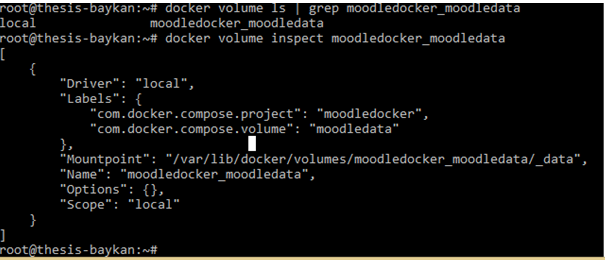
\includegraphics[width=14cm, height=7cm]{v_moodledata.png}
	\caption{Volume for moodledata}
	\label{fig2}
\end{figure}


